% Designdarstellung.tex
\subsection{Designdarstellung}
Neben der Produktdarstellung ist eine zentrale Komponente des FreeDesign-Editors doe Designdarstellung.
Durch das Einbetten der Designdarstellung in die Produktdarstellung, sind beide Komponenten voneinander entkoppelt und nicht aufeinander angewiesen. Die Darstellung des Designs basiert ebenfalls auf dem \textit{SVG}-Format für welche exklusive \textit{ReactJS}-Komponenten bestehen.

Weiterhin bestehen Abhängigkeiten in den \textit{core}-Ordner. Neben Datenstrukturen zur Beschreibung des Designs, betrifft das auch Funktionalitäten zum Parsen von Designdateien, sowie geometrischer Operationen. 


\begin{figure}[H]
    \centering
    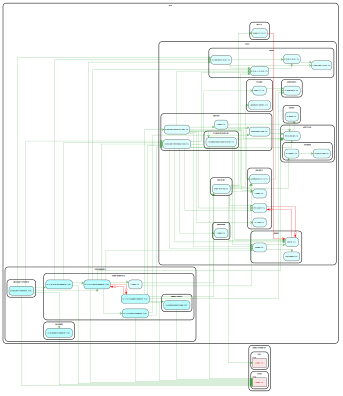
\includegraphics{diagrams/Ist-Architektur/design-presenter-analysis.pdf}
    \caption{Abhängigkeiten der Komponenten für Designdarstellung}
    \label{fig:Designdarstellung}
\end{figure}

\begin{enumerate}
\item Bildverarbeitung 
\item Cache 
\item Designdarstellung 
\item Designobjekt-Transformation 
\item Designobjekterzeugung 
\item Designstruktur 
\item Farbstruktur 
\item JavaScript-Erweiterung 
\item Mathematik  
\item Maßeinheit-Konverter 
\item Produktstruktur 
\item Schriftverarbeitung 
\item SVG-Parser 
\item XML-Parser 
\end{enumerate}
